\documentclass[a4paper,12pt]{article}
\usepackage[top = 2.5cm, bottom = 2.5cm, left = 2.5cm, right = 2.5cm]{geometry}
\usepackage[T1]{fontenc}
\usepackage[utf8]{inputenc}
\usepackage{multirow} 
\usepackage{booktabs} 
\usepackage{graphicx}
\usepackage[spanish]{babel}
\usepackage{setspace}
\setlength{\parindent}{0in}
\usepackage{float}
\usepackage{fancyhdr}
\usepackage{amsmath}
\usepackage{amssymb}
\usepackage{amsthm}
\usepackage{natbib}
\usepackage{graphicx}
\usepackage{subcaption}
\usepackage{booktabs}
\usepackage{etoolbox}
\usepackage{apalike}
\usepackage{minibox}
\usepackage{hyperref}
\usepackage{xcolor}
\usepackage{tcolorbox}
\usepackage{pdfpages}
\AtBeginEnvironment{align}{\setcounter{equation}{0}}
\newenvironment{solution}
  {\renewcommand\qedsymbol{$\square$}\begin{proof}[\textcolor{blue}{Solución}]}
  {\end{proof}}

\pagestyle{fancy}

\fancyhf{}

\lhead{\footnotesize Estadística 2}
\rhead{\footnotesize  Rudik Roberto Rompich}
\cfoot{\footnotesize \thepage}

\begin{document}
    \thispagestyle{empty} 
    \begin{tabular}{p{15.5cm}}
    \begin{tabbing}
    \textbf{Universidad del Valle de Guatemala} \\
    Departamento de Matemática\\
    Licenciatura en Matemática Aplicada\\\\
   \textbf{Estudiante:} Rudik Roberto Rompich\\
   \textbf{E-mail:} \textcolor{blue}{ \href{mailto:rom19857@uvg.edu.gt}{rom19857@uvg.edu.gt}}\\
   \textbf{Carné:} 19857
    \end{tabbing}
    \begin{center}
        MM2040 - Estadística 2 - Catedrático: Eugenio Aristondo\\
        \today
    \end{center}\\
    \hline
    \\
    \end{tabular} 
    \vspace*{0.3cm} 
    \begin{center} 
    {\Large \bf Tarea 5
} 
        \vspace{2mm}
    \end{center}
    \vspace{0.4cm}
%---------------------------
%\begin{tcolorbox}[colback=gray!15,colframe=black!1!black,title=A nice heading]
%\end{tcolorbox}

%\fbox{lol}
%---------------------------

\section{Capítulo 12}
\subsection{Problema 6} 
\begin{tcolorbox}[colback=gray!15,colframe=black!1!black,title=Ejericicio extra]
Se resolvió en clase.
\end{tcolorbox}
La American Bankers Association recoge datos sobre el uso de tarjetas de crédito o débito, cheques personales y efectivo para el pago de compras en tienda (The Wall Street Journal, 16 de diciembre de 2003). En 1999 los datos encontrados fueron los siguientes.
\begin{center}
    
\includegraphics[scale=0.5]{images/Screen Shot 2021-05-10 at 22.48.14.png}
\end{center}
En una muestra tomada en 2003 se encontró que de cada 220 compras en tienda, en 46 se usó tarjeta de crédito, en 67 tarjeta de débito, en 33 cheque personal y en 74 pago en efectivo.

\begin{enumerate}
    \item a) Con $\alpha=$ 0.01, ¿se puede concluir que en este periodo de cuatro años, de 1999 a 2003, se ha generado un cambio en la manera en que los clientes pagan sus compras en las tiendas? ¿Cuál es el valor-p?
    \begin{solution} Se considera la prueba de hipótesis: 
    \begin{align*}
        H_0: & 
             \text{ la población tiene una distribución multinomial con la}\\
            & \text{ probabilidad específica de cada una de las $k$ categorías.}\\
        H_a: &  
             \text{ la población no tiene una distribución multinomial con la}\\
         &\text{ probabilidad específica de cada una de las $k$ categorías.}
    \end{align*}
    
    Se considera el análisis hecho en Geogebra:
    
    \begin{center}
    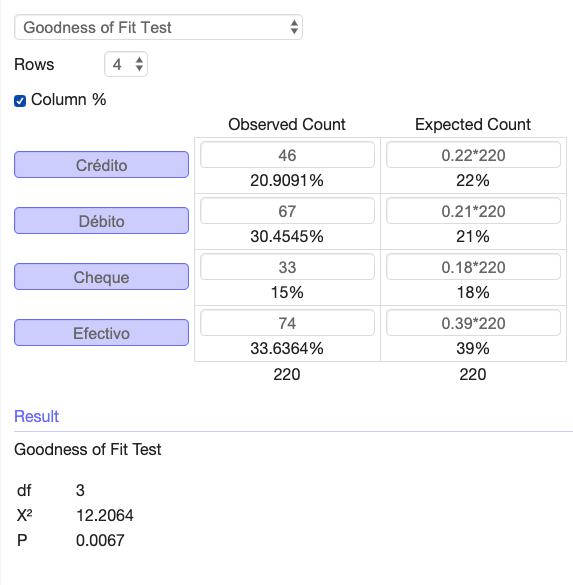
\includegraphics[scale=0.5]{images/Screen Shot 2021-05-10 at 23.15.45.png}
\end{center}
\begin{enumerate}
    \item El valor-p es 0.0067.
    \item Por el método del valor-p: $0.0067<0.01$; por lo que se puede concluir que de 1900 a 2003 sí se ha generado un cambio en el que los clientes pagan sus compras.
\end{enumerate}
    \end{solution}
\item b) A partir de los datos muestrales de 2003, calcule el porcentaje de uso de cada método de pago. ¿Cuál parece haber sido el principal o los principales cambios ocurridos en este período de cuatro años?
\begin{solution}
Los porcentajes se observan en la imagen de arriba. El cambio principal es el pago con tarjeta de débito, que subió de 21\% a aproximadamente 30.45\%
\end{solution}
\item c) ¿Qué porcentaje de los pagos se efectuó con tarjeta (de crédito o de débito) en 2003?
\begin{solution}
$$20.9091\%+30.4545\%= 51.36\%$$
\end{solution}
\end{enumerate}

\subsection{Problema 12} 

Visa Card USA estudió la frecuencia con que los consumidores de diversos rangos de edad usan tarjetas plásticas (de crédito o de débito) para pagar sus compras (Associated Press, 16 de enero de 2006). A continuación se presentan los datos muestrales de 300 clientes divididos en cuatro grupos de edad.

\begin{center}
    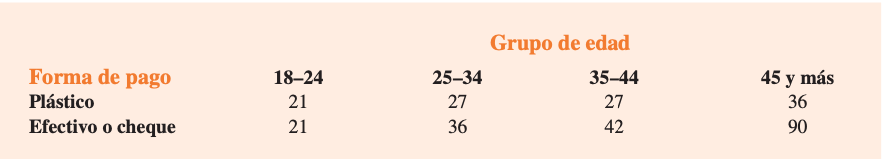
\includegraphics[scale=0.5]{images/Screen Shot 2021-05-10 at 23.28.28.png}
\end{center}


\begin{enumerate}
    \item a) Pruebe la independencia entre el método de pago y el grupo de edad. ¿Cuál es el valor-p? Usando $\alpha=$ 0.05, ¿cuál es su conclusión?
\begin{solution} Se considera la prueba de hipótesis: 
\begin{align*}
    H_0: & \text{ la variable de las columnas es independiente de la variable de las filas.}\\ 
    H_a: & \text{  la variable de las columnas no es independiente de la variable de las filas.}
\end{align*}
Se considera el análisis hecho en Geogebra:
\begin{center}
    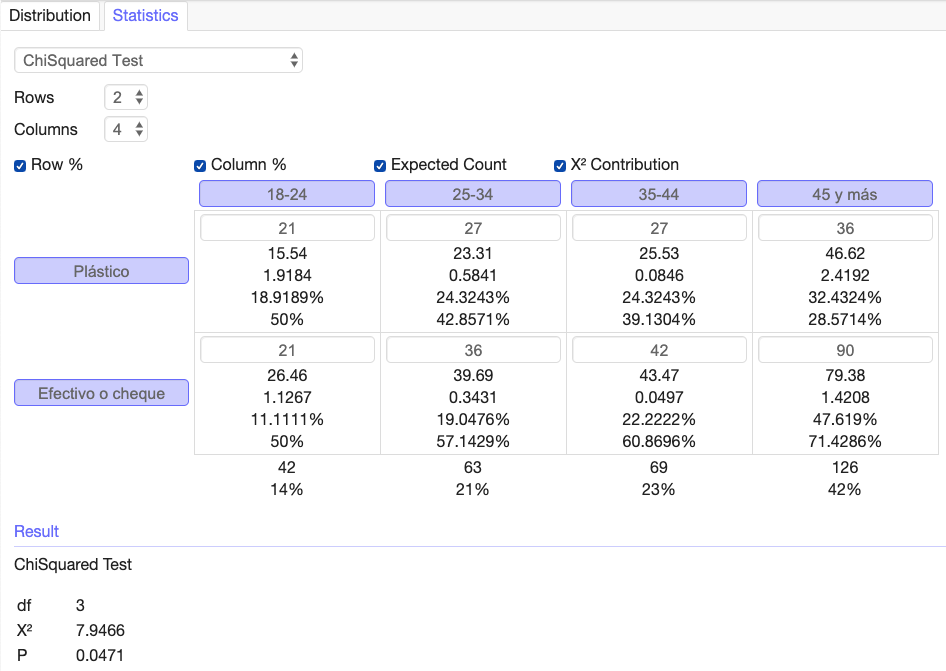
\includegraphics[scale=0.4]{images/Screen Shot 2021-05-10 at 23.40.36.png}
\end{center}

\begin{enumerate}
    \item El valor-p es 0.0471.
    \item Usando $\alpha=0.05$, por la prueba del valor-p $0.0471<0.05$ por lo que $H_0$ se rechaza. Hay evidencia suficiente para afirmar que grupo de edad no es independiente de las formas de pago. 
\end{enumerate}
\end{solution}
    \item b) Si la forma de pago y el grupo de edad no son independientes, ¿qué observación puede formular acerca de la diferencia en el uso del plástico en los diversos grupos de edad?
    \begin{solution}
    Las conclusiones son diversas, pero se puede observar que entre el grupo de personas es más joven, existe una preferencia en el plástico.
    \end{solution}
    \item c) ¿Qué consecuencias tiene este estudio para empresas como Visa, MasterCard y Discover?
    \begin{solution}
    Las consecuencias son variadas, pero pareciera indicar que estas compañías deberían enfocar en el uso del plástico a los grupos más viejos. 
    \end{solution}
\end{enumerate}


\subsection{Problema 15} 

FlightStats, Inc. recolecta datos sobre el número de vuelos programados y realizados en los principales aeropuertos de Estados Unidos. Sus datos indican que 56\% de los vuelos programados en los aeropuertos de Newark, La Guardia y Kennedy se efectuaron durante una tormenta de nieve que duró tres días (The Wall Street Journal, 21 de febrero de 2006). Todas las aerolíneas afirman que operan siempre dentro de parámetros de seguridad establecidos: si las condiciones son muy malas, no vuelan. Los datos en la tabla superior de la siguiente página presentan una muestra de 400 vuelos programados durante tormentas de nieve.
\begin{center}
    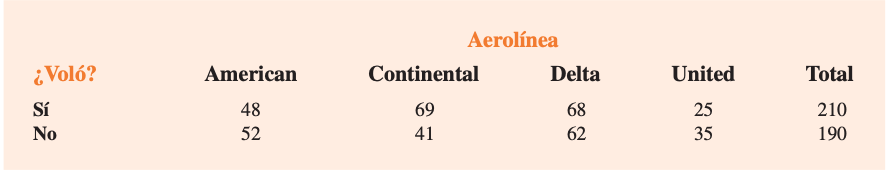
\includegraphics[scale=0.5]{images/Screen Shot 2021-05-11 at 00.03.21.png}
\end{center}

Use la prueba de independencia ji-cuadrada con un nivel de significancia de 0.05 para analizar estos datos. ¿Cuál es su conclusión? ¿Qué aerolínea elegiría para volar en condiciones de tormentas de nieve semejantes? Explique.

\begin{solution} 

Primero se consideran las hipótesis: 
\begin{align*}
    H_0: & \text{ la variable de las columnas es independiente de la variable de las filas.}\\ 
    H_a: & \text{  la variable de las columnas no es independiente de la variable de las filas.}
\end{align*}

Ahora bien, se considera el análisis hecho en Geogebra: 
\begin{center}
    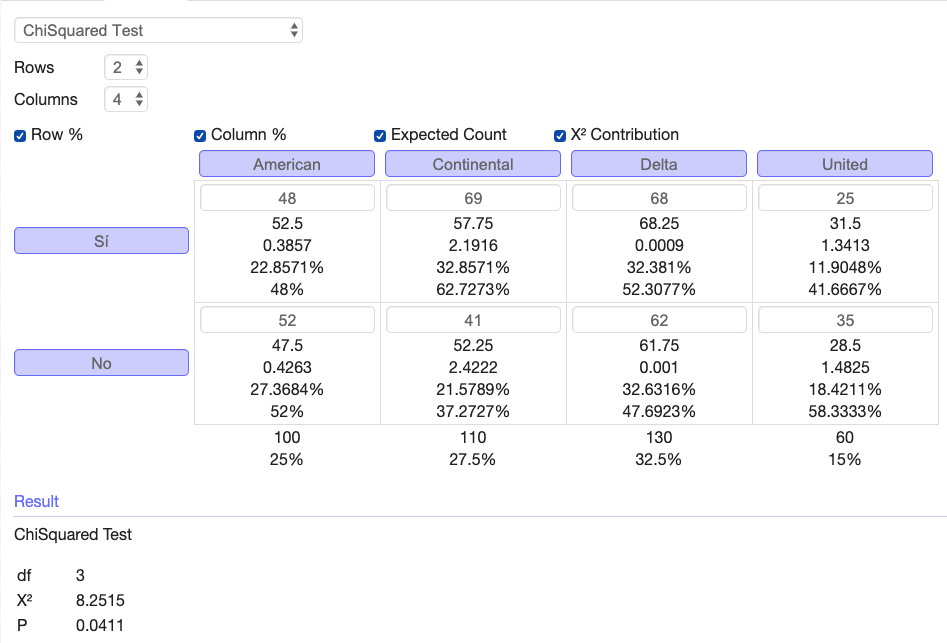
\includegraphics[scale=0.45]{images/Screen Shot 2021-05-11 at 00.13.22.png}
\end{center}
\begin{enumerate}
    \item El valor-p es 0.0411.
    \item Usando $\alpha=0.05$, por la prueba del valor-p $0.0411<0.05$ por lo que $H_0$ se rechaza. Hay evidencia suficiente para afirmar que la aerolínea no es independiente de si voló o no voló durante una tormenta de nieve. 
    \item En un primera vistazo, elegiría entre Delta y Continental; sin embargo, me decidiría por Continental; ya que tiene una menor cantidad de vuelos que no volaron comparado a Delta. 
\end{enumerate}
\end{solution}



\subsection{Problema 20} 

A continuación se presenta el número de ocurrencias por periodo y su frecuencia observada. Use $\alpha=$ 0.05 y la prueba de bondad de ajuste para determinar si estos datos se ajustan a una distribución de Poisson.
\begin{center}
    
\includegraphics[scale=0.45]{images/Screen Shot 2021-05-11 at 11.46.10.png}
\end{center}
\begin{solution}
Primero, se hacen los cálculos pertinentes con Excel, usando la distribución de Poisson definida como: 

$$f(x)=\frac{\mu^xe^{-\mu}}{x!}$$

Por lo cual, se tiene: 
\begin{center}
    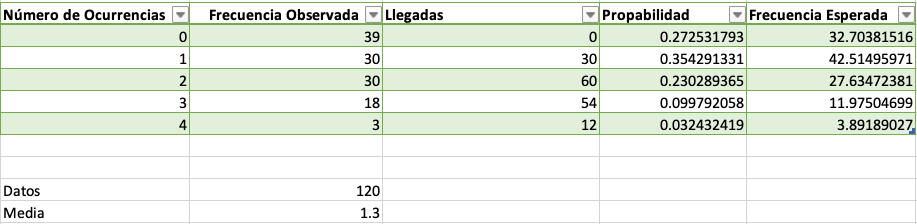
\includegraphics[scale=0.45]{images/Screen Shot 2021-05-11 at 11.47.16.png}
\end{center}

Definimos las hipótesis: 

\begin{align*}
    H_0: & \text{ la población tiene una distribución de Poisson.}\\ 
    H_a: & \text{  la población no tiene una distribución de Poisson.}
\end{align*}

Usando Geogebra: 

\begin{center}
    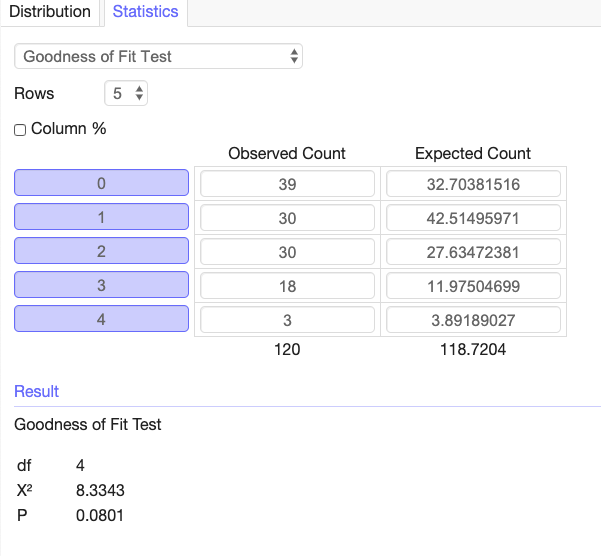
\includegraphics[scale=0.45]{images/Screen Shot 2021-05-11 at 11.49.48.png}
\end{center}

\begin{enumerate}
    \item El valor-p es 0.0801. 
    \item Por el método del valor-p: $0.0801>0.05$; por lo que $H_0$ no se rechaza. Por lo tanto, podemos concluir que los datos sí se ajustan a una distribución de Poisson.
\end{enumerate}
\end{solution}




\subsection{Problema 25} 

Use $\alpha=$ 0.01 y realice una prueba de bondad de ajuste para comprobar si la siguiente muestra fue tomada de una distribución normal.

\begin{center}
    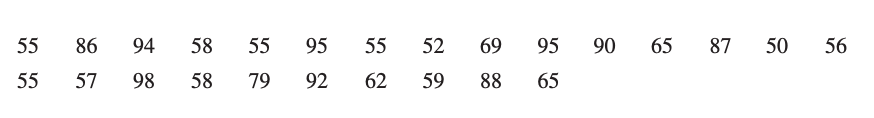
\includegraphics[scale=0.45]{images/Screen Shot 2021-05-11 at 11.56.58.png}
\end{center}

Una vez realizada la prueba de bondad de ajuste, elabore un histograma con todos estos datos. ¿Este gráfico respalda la conclusión a la que se llegó con la prueba de bondad de ajuste? (Nota. $\overline{x}=$ 71 y $s$ = 17.)
\begin{solution}Debido a la falta de instrucciones del problema, se propondrá distribuir la muestra en intervalos de 20\%, es decir que tendremos 5. Se propone utilizar Excel para esta tarea, con el comando
$$NORM.INV()$$
Por lo que tenemos: 
\begin{center}
    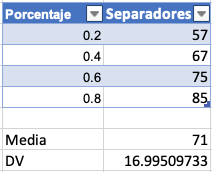
\includegraphics[scale=0.4]{images/Screen Shot 2021-05-11 at 14.43.01.png}
\end{center}
Ahora bien, considerando el análisis de histograma de Excel, tenemos: 
\begin{center}
    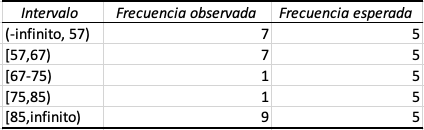
\includegraphics[scale=0.6]{images/Screen Shot 2021-05-11 at 14.46.58.png}
\end{center}

Usando Geogebra: 

\begin{center}
    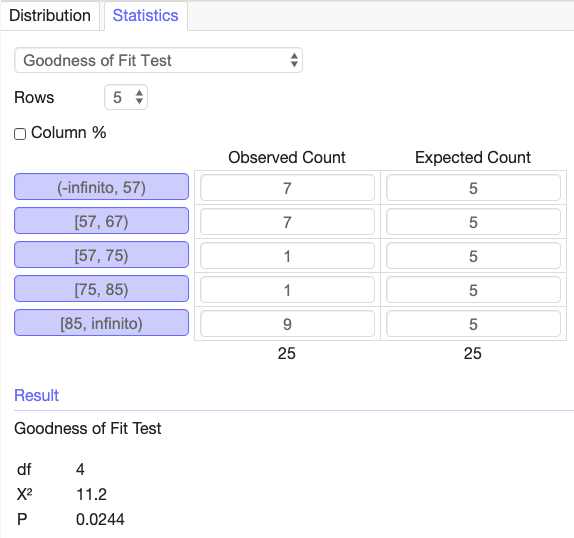
\includegraphics[scale=0.4]{images/Screen Shot 2021-05-11 at 15.05.35.png}
\end{center}
Se plantean las hipótesis: 
\begin{align*}
    H_0: & \text{ la población tiene una distribución normal.}\\ 
    H_a: & \text{  la población no tiene una distribución normal.}
\end{align*}

\begin{enumerate}
    \item El valor-p es 0.0244. 
    \item Por lo tanto, considerando la prueba del valor-p: 0.0244>0.01. Es decir que $H_0$ se acepta, entonces los datos tienen una distribución normal con una significancia de 0.01 . 
    \item El histograma: 
    \begin{center}
    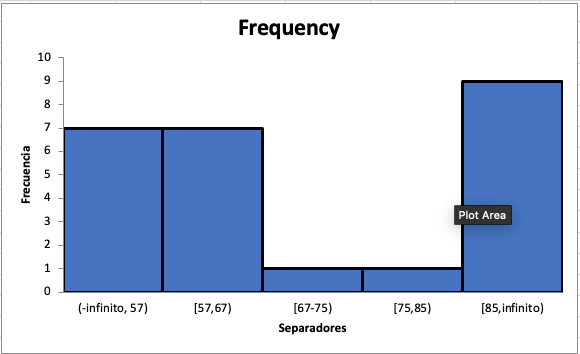
\includegraphics[scale=0.4]{images/Screen Shot 2021-05-11 at 15.19.10.png}
\end{center}
 El histograma no es de mucha ayuda, ya que a simple vista hace pensar que los datos no tienen un distribución normal; pero la conclusión de que los datos tienen una distribución normal es debido a la significancia que nos da el problema ($\alpha=$0.01); ya que con una significancia de 0.05 sí hubiera sido posible rechazar la $H_0$.
\end{enumerate}

\end{solution}

\begin{tcolorbox}[colback=gray!15,colframe=black!1!black,title=Segunda parte]
La segunda parte se hizo completamente en R-Markdown.
\end{tcolorbox}

\newpage 

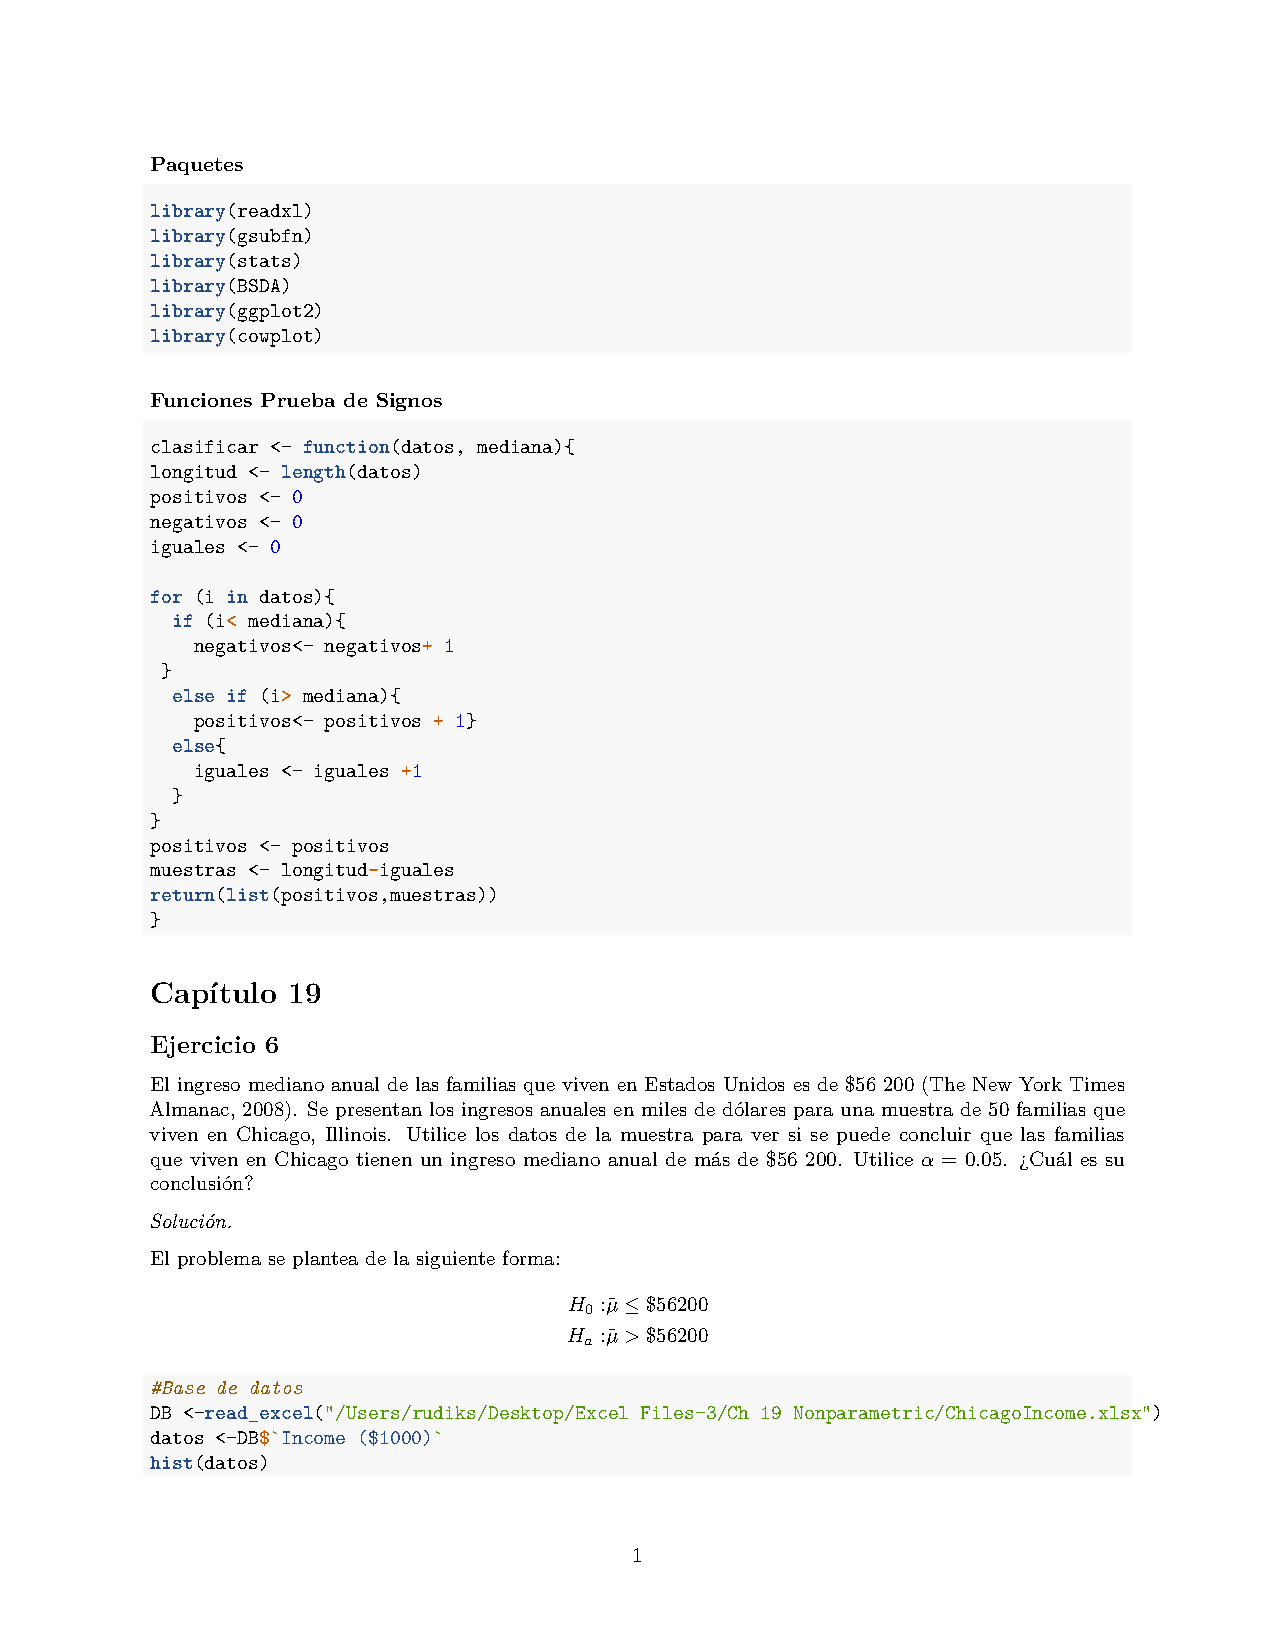
\includepdf[pages=-]{sec.pdf}


%---------------------------
%\bibliographystyle{apalike}
%\bibliography{sample.bib}

\end{document}